%Gesammtübersicht Fragestellung
Während der Messwoche der geophysikalischen Geländeübungen wurden vier verschiedenen Messmethoden verwendet, die Refraktionsseismik, Geoelektrik, Gravimetrie und Magnetik. An erster Stelle stand bei
uns die Fragestellung in wieweit sich die Ergebnisse dieser Messmethoden unterscheiden. Dadurch wollten wir die Messverfahren besser verstehen und einschätzen können welchen Einfluss die Wahl des Messverfahrens auf die Ergebnisse hat.

Wie bereits im Abschnitt Messgebiet beschrieben, wird unter Messgebiet 1 ein Basaltgang vermutet. Unser zweites Ziel war es, dessen Lage möglicht genau zu bestimmen. 


Wir wussten zwar, dass der Basaltgang eigentlich nicht mit der Seismik vermessen werden kann,
wollten dies aber Überprüfen und herausfinden in wiefern unsere Messergebnisse durch den Basaltgang beeinflusst worden sein könnten. Das Profil auf dem die Messung durchgeführt wurde ist in 
Abbildung \ref{abb:Seismik} als S21-S22 zu sehen.
Die Seismikmessung auf Messgebiet 2 wurde durchgeführt, um ein Verfahren zu haben mit dem die geoelektrikmessung verglichen werden kann und um gute Ergebnisse für die Auswertung zu haben.
Das Profil S31-S32 auf Messgebiet 2 war relativ lang und eben,wie man in Abbildung \ref{abb:Seismik} erkennt, so das wir davon ausgingen hier gut eine Schichtgrenze finden zu können.

\begin{figure}
 \centering
 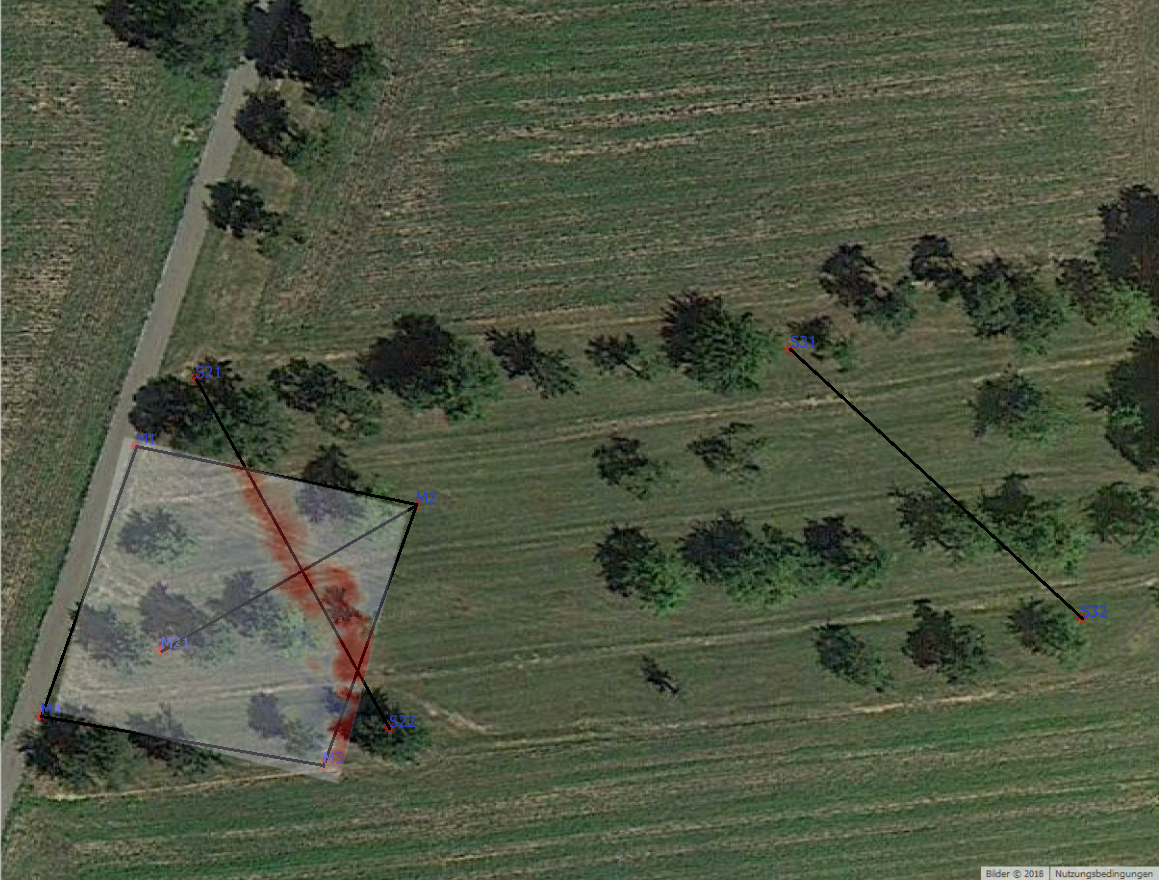
\includegraphics[width=0.9\textwidth]{fig/Seismik.png}
 \caption[Die Seismik- Messprofile S11-S21, S21-S22]{Die Seismik- Messprofile S11-S21, S21-S22. Die Graphik wurde von Rebekka Kirchgässner und Luisa Rank übernommen.}
\label{abb:Seismik}
\end{figure}

Die Magnetig wurde am ersten Tag durchgeführt. Hier war es uns bei der Kartierung wichtig zunächst die Lage des Basaltgangs festzustellen, um alle weiteren Messungen durchführen zu können.
Das Gebiet, auf dem die Kartierung zu sehen ist, ist in Abbildung \ref{abb:Kart} abgebildet. Die restlichen Messungen wurden auf den Profilen, die in Abbildung \ref{abb:Magnetig} eingezeichnet durchgeführt.
Hier war unsere Fragestellung wieder wie gut sich die Magnetik im Vergleich zu den anderen Messverfahren zu lokalisieren des Basaltgangs eignet.

\begin{figure}
 \centering
 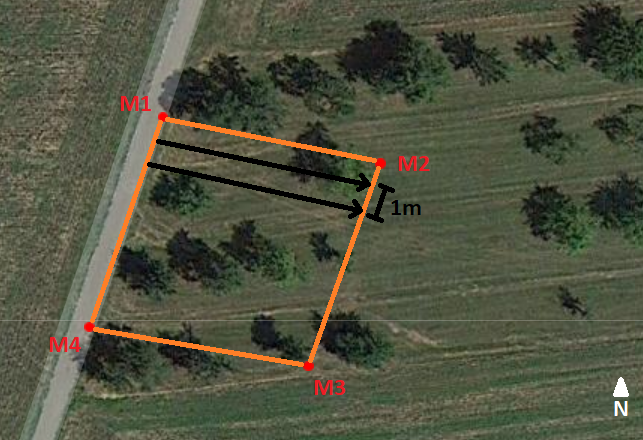
\includegraphics[width=0.9\textwidth]{fig/Kartierunggps.png}
 \caption[{Lage der Magnetk-Kartierung]{Lage der Magnetk-Kartierung. Die Graphik wurde von Rebekka Kirchgässner und Luisa Rank übernommen.}
 \label{abb:Kart}
\end{figure}

\begin{figure}
 \centering
 \includegraphics[width=0.9\textwidth]{fig/MagnetikGesammtueberblick.png}
 \caption[Gesammtübersicht über die Profile der Magnetig]{Gesammtübersicht über die Profile der Magnetig. Die Graphik wurde von Rebekka Kirchgässner und Luisa Rank übernommen.}
 \label{abb:Magnetik}
\end{figure}

Bei der Geoelektrik wurde wieder auf beiden Messgebieten eine Messung durchgeführt. Die Sondierung wurde auf einem Profil über dem der Seismik am Messgebiet 2 durchgeführt, dies ist in 
Abbildung ... eingezeichnet. Die Messung wurde durchgeführt um zu sehen ob wir Schichtgrenzen finden, und wenn ja ob diese mit denen der Seismik übereinstimmen.
Die Tomographie und Wenner-kartierung, Profil E11-E12, wurde wie schon Messungen der Magnetik und Gravimetrie orthogonal zum Basaltgang durchgeführt, um die Messergebnisse dieser drei Verfahren
miteinander vergleichen zu können. Die beiden Profile sind in Abbildung \ref{abb:Geoelek} abgebildet.

\begin{figure}
 \centering
 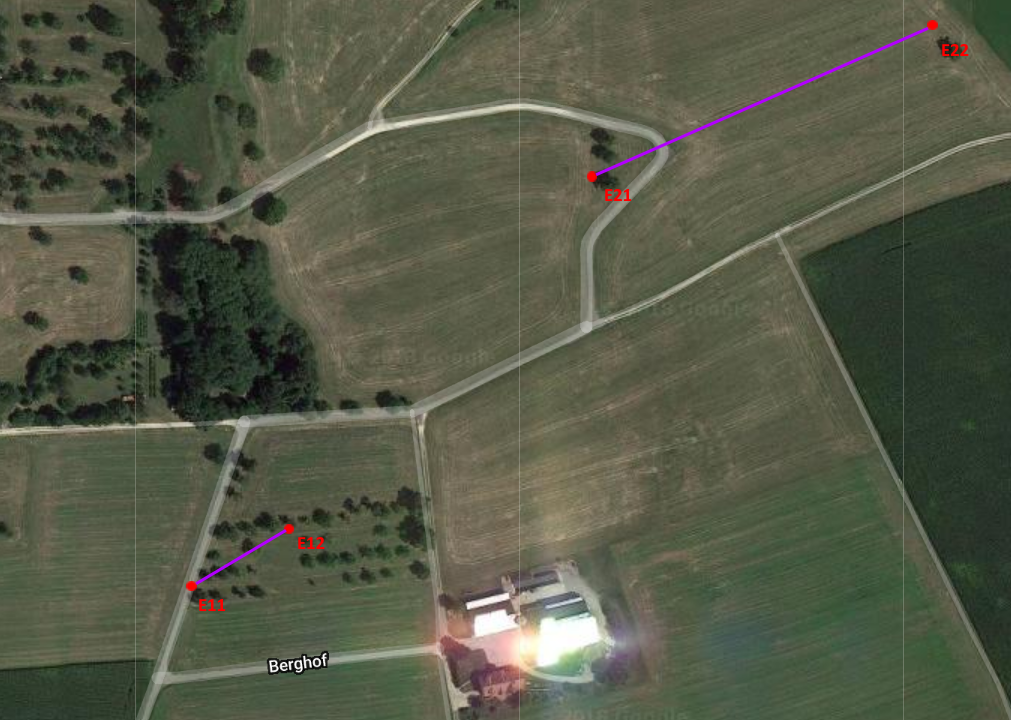
\includegraphics[width=0.9\textwidth]{fig/profilegps.png}
 \caption[Profile der Geoelktrik]{Profile der Geoelektrik. Die Graphik wurde von Rebekka Kirchgässner und Luisa Rank übernommen. }
 \label{abb:Geoelek}
\end{figure}

Da die Gravimetrie-Messung sehr viel Zeit in gebraucht hat, wurde nur eine Messung, auf Profil G11-G12, zu sehen in Abbildung \ref{abb:Geoelek2}, durchgeführt. Wir haben gehofft genau genug
messen zu können um den Basaltgang zu sehen und eventuell ähnliche Ergebnisse wie die bereits beschriebenen Messmethoden zu haben.

\begin{figure}
 \centering
 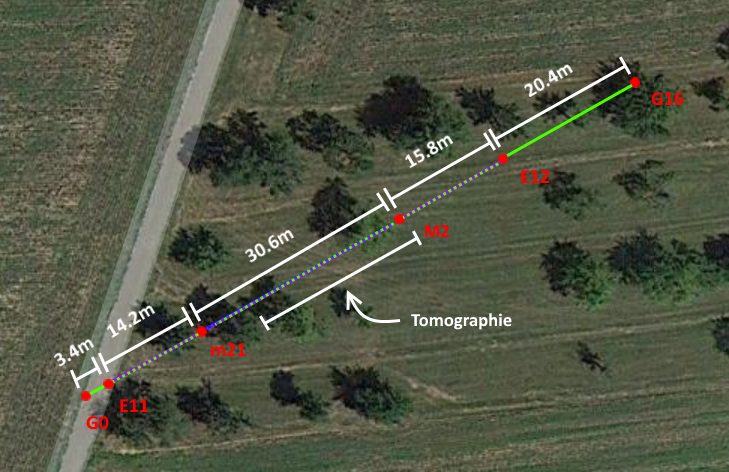
\includegraphics[width=0.9\textwidth]{fig/ElektrikMagnetikGravimetrie0gps.png}
 \caption[Profil der Gravimetrie]{Profil der Gravimetrie. Die Graphik wurde von Rebekka Kirchgässner und Luisa Rank übernommen. }
 \label{abb:Geoelek2}
\end{figure}






